\chptr{Termodimaica - Parte II}
\marginpar{\minitoc}

\epigraph{A: ``Quindi non è possibile nemmeno teoricamente?''\\I: ``Esattamente.''\\A: ``Per questo secondo me è \emph{mind-blowing}.''}{Una lezione di termodinamica,\\se non sbaglio sul II principio,\\a.a. 2023/2024, semestre II}

Lasciando stare per un momento il noioso capitolo precedente,
questa seconda parte è una sorta di storia piena di personaggi
leggendari, macchine e teorie bizzarre; qualcosa che tocca
quasi il genere steampunk. Ora che abbiamo in mano gli strumenti
fondamentali della termodinamica, possiamo vedere nel
dettaglio le applicazioni e le implicazioni di questa viverna
fatta di energia allo stato puro, aggiungendo però altri
principi fondamentali. Rispetto a molti altri
argomenti di questo corso (e della fisica stessa), questo
capitolo sottolinea come in realtà la scienza non sia
solamente alla ricerca di cosa si può fare, ma anche di
cosa è impossibile e quali limiti ci tocca accettare. Uno
di questi è il seguente: una
volta innescato un fenomeno, non sempre si può tornare indietro.
Scopriremo alla fine che questa osservazione è strettamente
legata alla nostra percezione dello scorrere del tempo.

\section{Macchine}


\subsection{Rendimento}
Ora che abbiamo costruito la nostra macchina, ci chiediamo quanto ci
costi mantenerla in funzione, ovvero quanta energia richiede (la quantità
di combustibile ad esempio) e quanta di questa energia viene utilizzata
senza essere sprecata. In un motore di un'auto, per esempio, vorremmo che
tutta, o quasi tutta, la benza venga consumata per permetterci di raggiungere
Povo da Trento senza intoppi, anche se sappiamo che l'auto si scalda, il pistone
e le ruote fanno attrito frenando di un po' la nostra corsa e così via.
In altre parole, ci stiamo ponendo il problema
di determinare l'efficienza della macchina, chiamata anche rendimento.


\subsection{Ciclo Diesel e ciclo di Otto}
Esaminiamo un esempio reale di ciclo termodinamico, impiegato in
una classe diffusa di motori termici: il ciclo Diesel, il cui
principio di funzionamento consiste nel portare la mistura di
miscela e aria a pressione elevata in tempi brevi per generare
lo scoppio. Tale ciclo
è illustrato sul piano $pV$ nella figura \ref{erciclodiesel}, anche
se in realtà, come vedremo, si tratta solo di una spensierata idealizzazione.
Considereremo infatti molti tratti del ciclo come trasformazioni
quasistatiche. Nel ciclo, il gas che subisce queste trasformazioni
è il mix di aria, combustibile (la cosiddetta miscela) ed
eventuali residui di scarico, combusti o meno.
Il ciclo diesel è costituito dai seguenti tratti, o
``tempi'':

\begin{marginfigure}
    \centering
    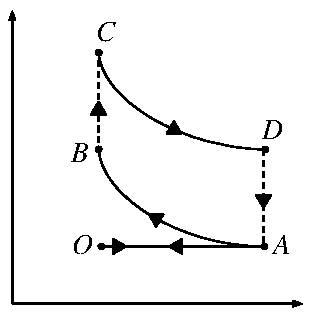
\includegraphics[width = \marginparwidth]{ciclo_diesel.pdf}
    \caption{Ciclo diesel teorico.}
    \label{erciclodiesel}
\end{marginfigure}

\begin{enumerate}
    \item $OA$ è una fase di aspirazione della miscela. Si
    tratta di una trasformazione isobara. Qui il pistone si
    abbassa, aumentando il volume della camera di combustione.

    \item $AB$ è una adiabatica, che corrisponde ad una compressione
    forte abbastanza da innescare, in $B$, l'esplosione della
    miscela. Ovviamente non viene scambiato calore.

    \item $BC$ è la fase di esplosione. Si tratta di un fenomeno
    più complesso di quello che i nostri strumenti di termodinamica
    possano descrivere. Per questo assumiamo che tale fase non
    sia quasistatica, essendo tra l'altro molto rapida. Questo tratto
    è quello che immette calore
    nel cilindro, permettendo di alzare violentemente la pressione
    (e la temperature) a volume idealmente costante.

    \item $CD$ è una seconda adiabatica, nella quale il pistone
    viene spinto in seguito alla precedente esplosione. Qui viene
    compiuto lavoro dal motore.

    \item $DA$ è un'altra fase non quasistatica, perché dopo le
    precedenti due fasi violente il pistone termina la sua
    corsa; pressione e temperatura crollano vertiginosamente.

    \item $AO$ chiude il ciclo, scaricando i gas combusti e,
    permettendo di preparare il motore all'aspirazione di miscela
    successiva.
\end{enumerate}

Calcoliamo l'efficienza di questo ciclo. Innanzitutto, posiamo
notare che le fasi $OA$ e $AO$, sommandosi, si annullano e dunque
non le considereremo. Possiamo utilizzare la definizione di
efficienza $\eta = 1 - |Q_c|/Q_a$; serve dunque calcolare i
calori scambiati nel ciclo. Dal momento che $AB$ e $CD$ sono
adiabatiche, rimangono solo i tratti $BC$ e $DA$. Abbiamo detto
che queste fasi non sono quasistatiche, ma possiamo notare che
avvengono dei ``salti'' di temperatura simili ad una isocora.
Facendo dunque finta di nulla, manco fossimo ad un attraversamento
pedonale col semaforo rosso per i pedoni,
possiamo supporre che valgano le leggi finora studiate:

\begin{align*}
    Q_a &= Q_{BC} = \Delta U_{BC} = nc_V(T_B - T_C) > 0\\
    Q_c &= Q_{DA} = nc_V(T_A - T_D) < 0
\end{align*}

\noindent da cui

\[ \eta_\text{Diesel} = 1 - \frac{|T_A - T_D|}{T_C - T_B} \]

\noindent ricordiamo, in condizioni ideali. Questa efficienza,
secondo analisi più approfondite, potrebbe raggiungere un
valore pari a $\eta \simeq 0.6$.

\begin{marginfigure}
    \centering
    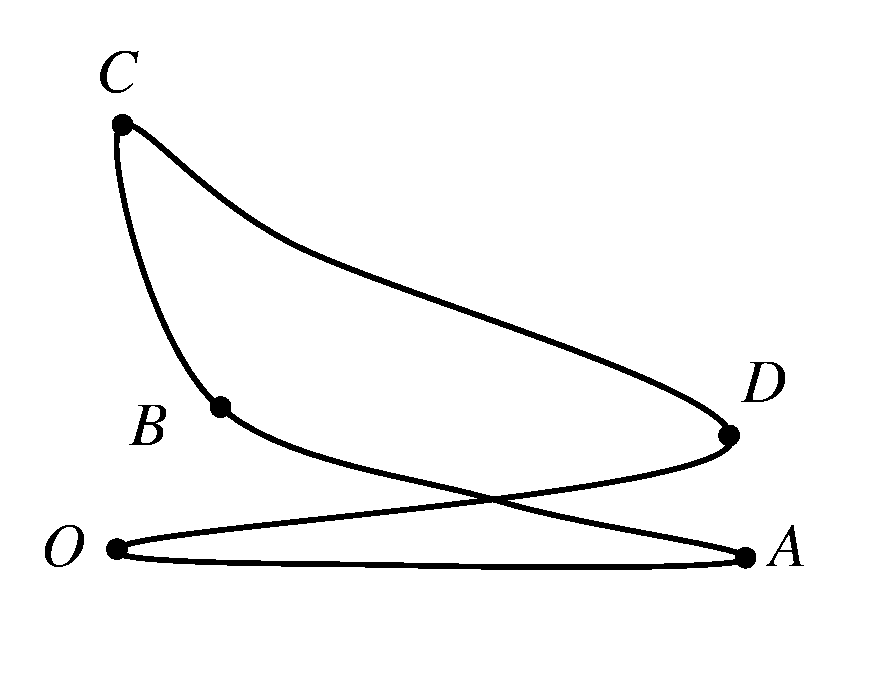
\includegraphics[width = \marginparwidth]{ciclo_8.pdf}
    \caption{Rappresentazione approssimativa del ciclo di Otto in
    condizioni reali. Sono evidenziate anche le coordinate teoriche
    corrispondenti a quelle presenti in figura \ref{erciclodiesel}.}
    \label{ciclo8}
\end{marginfigure}

Nella realtà, il ciclo Diesel come appena mostrato è ben lontano
da quelli che vengono solitamente progettati. In figura \ref{ciclo8}
viene mostrato il \textit{ciclo Otto}, molto simile a quello Diesel
e dal quale traggono ispirazione i maggiori tipi di motori termici
attuali. Si deve essere coscienti del fatto che la forma in figura
subisce numerosissime fluttuazioni sul piano $pV$ e l'intera trasformazione
è ovviamente irreversibile. Tutto ciò spiega il crollo drastico
dell'efficienza prevista teoricamente.






\section{Principio secondo}
Dopo aver introdotto il concetto di macchina e della sua efficienza,
è legittimo chiedersi se è possibile progettare nella realtà
la macchina perfetta, che cioè converte tutta l'energia
(in particolare calore) in ingresso interamente in lavoro in uscita,
con efficienza unaria (100\%).
Operando ciclicamente, per una macchina dovrebbe seguire dal primo
principio $\Delta U = Q - W$ la conclusione $\Delta U = 0$ e allora

\[ Q = W \]

\noindent La teoria sembrerebbe essere fondata: lavoro e calore sono
convertibili, cioè spendendo calore otteniamo lavoro e possiamo tra l'altro
invertire il processo, perché l'uguaglianza non ci impone un
verso preferenziale e noi siamo tanto furbi da costruire macchine
in grado di funzionare al contrario. Per esperienza, tuttavia, è evidente che non
è così, cioè se spendiamo una certa quantità di calore $Q$ e
la trasformiamo in lavoro, sembra impossibile, mediante quel lavoro,
riottenere tutto il calore $Q$ iniziale. Per fare un esempio, potremmo
immaginare di costruire un mulino ad acqua in questo modo: sappiamo che
tutti i mulini sono mossi dalla corrente e in tal modo producono
lavoro; potremmo dunque far sì che il mulino alimenti una pompa che
riporta l'acqua in cima al mulino, facendolo muovere indefinitamente.
Assumendo che il dispositivo sia costruito in maniera
eccellente, riducendo quanto possibile dispersione e attriti,
in realtà questa macchina è destinata a fermarsi dopo un certo
intervallo di tempo\footnote{Consigliamo di dare un'occhiata alla
sezione dedicata al moto perpetuo, negli approfondimenti di questo
capitolo.}, sia esso una manciata di secondi o qualche milione di
anni.

Potremmo ribattere affermando che la realtà ci pone problemi come
attrito e dissipazioni di vario genere. Ciò che è sconcertante è
l'impossibilità non solo reale di costruire macchine simili,
ma anche teorica. Questa conclusione, come vedremo, fonda
le radici nel secondo principio, che a sua volta poggia sulla
seguente evidenza:

\begin{center}
    \textit{il calore non fluisce \underline{\emph{mai spontaneamente}} da un corpo ad uno più caldo}.
\end{center}

\subsection{Enunciati}
Esistono due enunciati celebri del secondo principio della termodinamica\footnote{Anche se storicamente non fu così, trattiamo prima l'attuale forma
del secondo principio della termodinamica, permettendoci di chiarire
le sezioni successive.}.
In qualità di principi, essi sono dati per veri sulla base dell'esperienza,
ma è comunque possibile dimostrare che essi si riferiscono alla
stessa proprietà della natura.

\begin{tcolorbox}[colback = red!30, colframe = red!30!black, title = {Enunciati del secondo principio della termodinamica}]
    \begin{itemize}
        \item \textbf{Enunciato di Kelvin-Plank}
        
        \begin{center}
            \textit{È impossibile realizzare una macchina il cui unico risultato
            sia quello di trasformare calore, a partire da una sola sorgente, interamente in lavoro.}
        \end{center}
    
        \item \textbf{Enunciato di Clausius}
        
        \begin{center}
            \textit{È impossibile realizzare un processo il cui unico risultato\\
            sia quello di trasferire calore da un corpo ad uno più caldo.}
        \end{center}
    \end{itemize}
\end{tcolorbox}

\noindent Una delle proprietà della natura che il secondo principio sottointende
è il fatto che ogni macchina termica, qualsiasi essa sia (anche tra quelle non ancora
inventate!) deve sempre operare tra almeno due sorgenti affiché essa possa
funzionare. Inoltre, da come si evince dall'enunciato di Kelvin-Plank, è impossibile
costruire macchine con rendimento pari a 1.

\subsection{Equivalenza degli enunciati}
Dimostreremo che i due enunciati sono equivalenti nel seguente modo:
indicando con $KP$ l'enunciato di Kelvin-Plank e con $C$ quello di
Clausius, concluderemo che $KP \Leftrightarrow C$ mostrando che
$\overline{KP} \Leftrightarrow \overline{C}$, cioè negando l'uno necessariamente
si deve negare anche l'altro\footnote{Dimostrazione: siano $a,b$ affermazioni
tali che $a \Leftrightarrow b$. Allora $(a \Leftrightarrow b) \equiv (a \Rightarrow b
\wedge b \Rightarrow a) \equiv (\lnot b \Rightarrow \lnot a \land \lnot a \Rightarrow \lnot b) \equiv (\lnot a \Leftrightarrow \lnot b)$,
dove nel terzo passaggio abbiamo impiegato la contronominale dell'implicazione $\Rightarrow$,
per cui $(x \Rightarrow y) \equiv (\lnot x \lor y) \equiv (\lnot\lnot\lnot x \lor \lnot\lnot y) \equiv (\lnot y \Rightarrow \lnot x)$.}. Di volta in volta
considereremo macchine che disobbediscono ai due principi, che chiameremo
sempre $\overline{KP}$ e $\overline{C}$, e che operano tra due
serbatoi 1 e 2 a temperature $T_1 < T_2$.

\subsubsection*{Dimostrazione: $\overline{KP} \Rightarrow \overline{C}$}
Cominciamo mostrando che $\overline{KP} \Rightarrow \overline{C}$,
facendo riferimento alla figura \ref{kptocproof}.
Consideriamo allora la macchina $\overline{KP}$ che preleva una
certa quantità di calore $Q_1 > 0$ da 1 e lo converte interamente
in lavoro $W$, alla facciaccia di Kelvin e Plank.

\[ Q_1 = W \]

\begin{marginfigure}
    \centering
    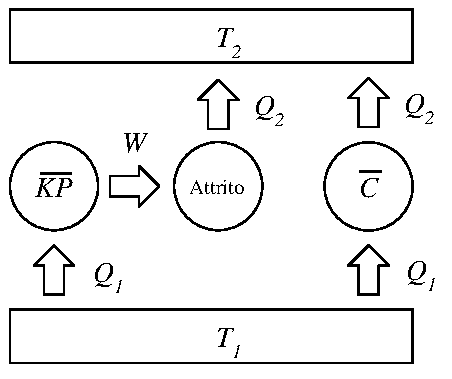
\includegraphics[width = \marginparwidth]{violare_kelvin-plank.pdf}
    \caption{Dimostrazione dell'implicazione $\overline{KP} \Rightarrow \overline{C}$.}
    \label{kptocproof}
\end{marginfigure}

\noindent Il lavoro $W$ viene poi impiegato per alimentare una
seconda macchina che cede il calore prodotto $Q_2$ alla sorgente
2. Questa macchina può essere progettata, per esempio, sulla base
di trasformazioni isoterme, oppure dissipando il lavoro meccanico
in attrito, che genera sempre calore. Allora

\[ Q_2 = -W \]

\noindent Ma allora,
se uniamo le macchine, ne otteniamo una che nel complesso preleva
del calore $Q_1$ dalla sorgente fredda 1 e cede quella stessa
quantità di calore alla sorgente calda 2, senza produrre altri
risultati. Questa macchina composta è proprio $\overline{C}$.

\begin{marginfigure}
    \centering
    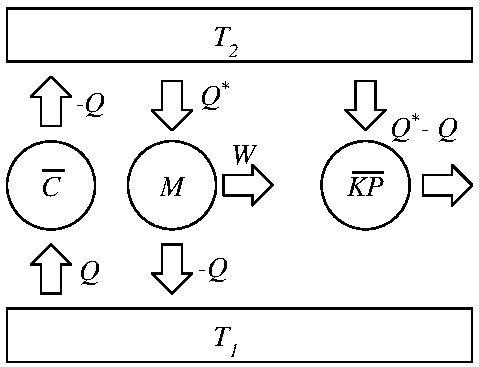
\includegraphics[width = \marginparwidth]{violare_clausius.pdf}
    \caption{Dimostrazione dell'implicazione $\overline{C} \Rightarrow \overline{KP}$.}
    \label{ctokpproof}
\end{marginfigure}

\subsubsection*{Dimostrazione: $\overline{C} \Rightarrow \overline{KP}$}
Si osservi la figura \ref{ctokpproof}.
Supponiamo di avere una macchina $\overline{C}$ che trasferisce
calore $Q > 0$ da 1 verso 2. Il calore in entrata nella macchina è
$Q_1 = Q$ mentre quello in uscita è $Q_2 = -Q$.
Consideriamo poi una seconda macchina $M$, progettata per prelevare
del calore $Q^* > Q$ dalla sorgente calda 2, produrre lavoro $W$
e cedere calore $Q_c = -Q$ alla sorgente fredda 1. Questo è ammissibile
operando sul rendimento $\eta_M = 1 - |Q_c|/Q^*$ di $M$.
Se si uniscono $\overline{C}$ e $M$, si ottiene una macchina che nel
complesso assorbe calore $Q^* - Q$ dalla sorgente calda 2, produce
lavoro $W$ ma che preleva per poi cedere di nuovo lo stesso calore
$Q$ alla sorgente 1, come se non esistesse. Dunque $W = Q^* - Q$.
La macchina composta corrisponde allora a $\overline{KP}$.

Si potrebbe ribattere sostenendo che $\overline{KP}$ può funzionare
perché vi è comunque scambio di calore $Q$ con la sorgente fredda,
anche se questo calore viene sempre ceduto e prelevato ripetutamente,
ma comunque questo ragionamento non regge. Per convincerci di ciò,
basta pensare ad un'altra macchina composta $X$ che incorpora
$\overline{KP}$ (costruita precedentemente) e la sorgente 1, mentre la 2
rimane esterna. Non vediamo la sorgente 1, in quanto componente
della macchina $X$ che opera solamente con la sorgente 2. Allora anche $X$
è analoga ad una macchina di tipo $\overline{KP}$.


\section{Esperienza di Carnot}
Nel 1824, l'ingegnere francese Sadi Carnot pubblicò il
\textit{Réflexions sur la puissance motrice du feu et sur les machines
propres à développer cette puissance}. Trascurando il titolo
altisonante, la questione che egli affrontò nell'opera
scaturì dalla nascente competizione alimentata dalla rivoluzione industriale:
In quali condizioni una macchina termica ha il redimento
massimo, indipendentemente da come essa viene costruita? Come
vedremo, la potenza di questa domanda (e della sua risposta) sta
proprio nell'indipendenza dalla tecnologia con la quale la
macchina funziona. Non importa se essa è il motore di una monoposto
di Formula 1, lo scramjet del Boeing X-43 o un altro metodo di
propulsione di qualche civiltà aliena a noi sconosciuta.

\begin{marginfigure}
    \centering
    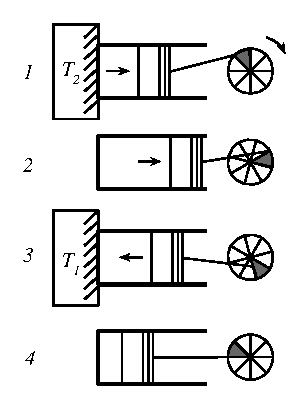
\includegraphics[width = \marginparwidth]{macchina_di_carnot.pdf}
    \caption{I quattro tempi che costituiscono il ciclo di funzionamento della macchina di Carnot.
    Il diagramma originale di Carnot non lo prevedeva, ma possiamo immaginare questa macchina come
    un classico motore che mette in rotazione un volano.}
    \label{macchinacarnot}
\end{marginfigure}

\subsection{Ciclo e macchina di Carnot}
Per rispondere ai suoi quesiti,
Carnot si ingegnò nella creazione di una macchina ideale,
la \textit{maccina di Carnot} (che indicheremo spesso con $\mathcal{C}$),
costituita da un cilindro che può esser reso adiabatico o
diatermico a piacere, un pistone mobile e un gas sottoposto al
\textit{ciclo di Carnot}. Altri componenti essenziali sono due
sorgenti a temperature differenti.
Un modello della macchina è mostrato in figura \ref{macchinacarnot}.
Durante un ciclo
di funzionamento, la macchina esegue i seguenti quattro passi
(consideriamo la sua versione termica, non frigorifera):


\begin{enumerate}
    \item \textit{Acquisizione di calore:} la macchina viene posta sulla
    sorgente calda. Supponendo che il gas sia già alla temperatura di
    questa sorgente, esso viene espanso isotermicamente, determinando
    il sollevamento del pistone e dunque la conversinoe di calore in
    lavoro.

    \item \textit{Raffreddamento adiabatico:} la macchina viene tolta dalla
    sorgente calda, ma il gas continua ad espandersi adiabaticamente
    (per questo il cilindro deve essere adiabatico durante questa
    fase) fino a raggiungere la temperatura della sorgente fredda.

    \item \textit{Cessione di calore:} il pistone viene abbassato per
    comprimere il gas, che isotermicamente cede calore alla sorgente
    fredda.

    \item \textit{Riscaldamento adiabatico:} la macchina viene tolta dalla sorgente
    fredda, ma il gas continua ad esser compresso adiabaticamente fino
    a raggiungere la temperatura della sorgente più calda. Il ciclo
    ricomincia.
\end{enumerate}

Carnot tiene a sottolineare come la macchina debba operare in condizioni
ben controllate, perché il gas al suo interno deve poter percorrere un
ciclo termodinamico \textit{quasistatico reversibile}. Perciò, lo spostamento
della macchina tra le due sorgenti, la compressione e l'espansione devono
essere estremamente lente, tanto da evitare attriti, dissipazioni di
calore, fluttuazioni irregolari nella temperatura delle sorgenti e del gas,
turbolenze e comportamenti non ideali delle particelle di gas.
Una volta certi di aver soddisfatto i requisiti appena citati, il
grafico del \textit{ciclo di Carnot} si presenterà nella forma mostrata
in figura \ref{ciclodicarnot}.

\begin{marginfigure}
    \centering
    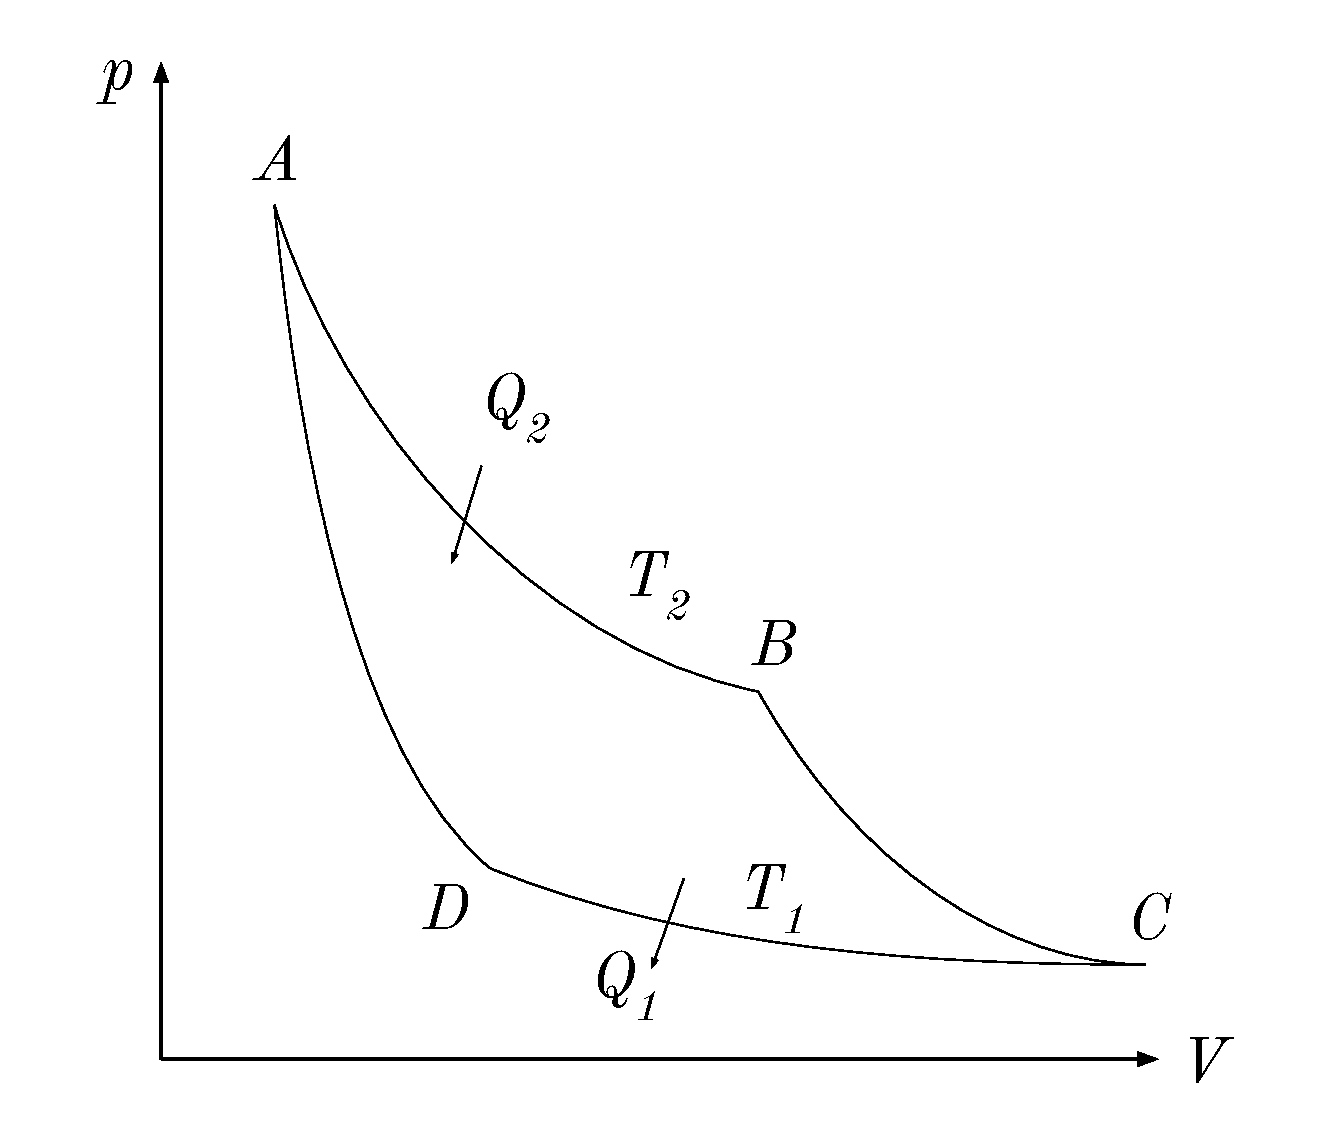
\includegraphics[width = \marginparwidth]{ciclo_di_carnot.pdf}
    \caption{Il ciclo di Carnot sul piano $pV$.}
    \label{ciclodicarnot}
\end{marginfigure}



Analizzando il ciclo otterremo un risultato interessante.
Supponiamo che la sorgente fredda abbia temperatura $T_1$ mentre quella
calda $T_2$ e che la macchina di Carnot venga caricata di $n$ moli
di gas ideale. Calcoliamo gli scambi di energia nelle varie
trasformazioni che compongono il ciclo:

\begin{itemize}
    \item \textit{AB:} essendo una isoterma, $\Delta U_{AB} = 0$ e
    \[ Q_{AB} = W_{AB} = nRT_2\ln\left(\frac{V_B}{V_A}\right) > 0 \]
    Notare come questo costituisce il calore assorbito dalla macchina.

    \item \textit{BC:} essendo adiabatica, $Q_{BC} = 0$ e
    \[ \Delta U_{BC} = -W_{BC} = -nc_V(T_1 - T_2) \]

    \item \textit{CD:} la situazione è analoga a quella in \textit{AB}:
    \[ Q_{CD} = nRT_1\ln\left(\frac{V_D}{V_C}\right) < 0 \]

    \item \textit{DA:} come in \textit{BC}
    \[ \Delta U_{DA} = -W_{DA} = -nc_V(T_2 - T_1) \]
\end{itemize}

\noindent Abbiamo potuto usare le leggi ricavate dallo studio delle
trasformazioni elementari perché abbiamo supposto che il ciclo di
Carnot fosse quasistatico-reversibile. Veniamo ora alla risposta che
Carnot desiderava trovare: quale efficienza può essere raggiunta da
una tale macchina. Applicando la definizione di rendimento, dai
risultati precedenti è facile concludere che

\[ \eta_\mathcal{C} = \frac{W}{Q_{AB}} = 1 + \frac{T_1}{T_2}\frac{\ln(V_D/V_C)}{\ln(V_B/V_A)} \]

\noindent Ricordando la legge \ref{lativuu} che caratterizza le
trasformazioni adiabatiche, si scopre che l'efficienza qui sopra può
essere semplificata ulteriormente. Infatti, per la trasformazione
\textit{BC} vale $T_2V_B^{\gamma - 1} = T_1V_C^{\gamma - 1}$ mentre
per \textit{DA} $T_1V_D^{\gamma - 1} = T_2V_A^{\gamma - 1}$. Mediante
semplice algebretta, è evidente che $V_B/V_A = V_C/V_D$. Concludiamo
allora che

\begin{align}
    \eta_\mathcal{C} = 1 - \frac{T_1}{T_2}
\end{align}

Ecco dunque svelato l'arcano: idealmente, l'efficienza di una buona
macchina, ovvero ideale, dipende unicamente dalle temperature entro
le quali essa opera. Quanto più la loro differenza è grande, tanto
più la macchina sarà efficiente. Tuttavia, allo stato attuale della
nostra conoscenza della natura, non possiamo neppur teoricamente
ottenere $\eta_\mathcal{C} = 1$, (anzi $0 \leq \eta_\mathcal{C} < 1$),
perché dovremmo possedere un oggetto di temperatura $T_2 = +\infty$\footnote{Ammesso che ciò possa essere fisicamente sopportabile da qualche materiale misterioso, un corpo a temperatura infinita sarebbe
caratterizzato da un'energia interna infinita, il che minerebbe la
solidità dei principi di conservazione fin ora incontrati.},
oppure un oggetto a temperatura nulla\footnote{Si faccia
riferimento agli approfondimenti di questo capitolo per giustificazioni
alternative dell'impossibilità di raggiungere lo zero assoluto.}.

Vale inoltre per una macchina di questo tipo

\[ 1 - \frac{T_1}{T_2} = 1 - \frac{|Q_\text{ced}|}{Q_\text{ass}} \]

\noindent per cui

\begin{align}
    \frac{T_1}{T_2} = \frac{|Q_\text{ced}|}{Q_\text{ass}}
\end{align}



\subsection{Teorema di Carnot}
Carnot progettò mentalmente una macchina semplice ma inrealtà
particolare, che ha ben poco a che fare con il motore, ad esempio,
di una turbina di un aereo. Per questo motivo è stato formulato
il teorema di Carnot, con il quale si estende la valutazione
dell'efficienza a \textit{tutte} le macchine che operano tra due
sole sorgenti, anche quelle non ancora progettate.


\begin{tcolorbox}[colback = red!30, colframe = red!30!black, title = {Teorema di Carnot}]
Il rendimento di una qualsiasi macchina termica $X$ (reversibile o non)
che opera tra due
temperature costanti $T_1,T_2: T_1 < T_2$ è limitato superiormente dal rendimento della
macchina di Carnot $\mathcal{C}$ che lavora tra le medesime temperature.

\begin{align}
    \eta_X \leq \eta_\mathcal{C} \quad \text{per } T_1 < T_2\label{carnot1}
\end{align}

Inoltre, tutte le macchine reversibili che operano con la stessa coppia di temperature
hanno lo stesso rendimento, che equivale a quello della corrispondente macchina di
Carnot. Se $X$ è una macchina reversibile, allora:

\begin{align}
    \eta_X = \eta_\mathcal{C}\label{carnot2}
\end{align}

\end{tcolorbox}


\subsubsection*{Dimostrazione}
Si faccia riferimento alla figura \ref{teo_carnot}.
Per dimostrare il teorema, consideriamo una macchina $X$ qualsiasi
e una macchina di Carnot $\mathcal{C}$. Esse operano tra le solite
sorgenti a temperature $T_1$ e $T_2 > T_1$.
$X$ è costruita in tal guisa da produrre lavoro $W'$ e scambiare
calore $Q_1' < 0$ e $Q_2' > 0$ con le rispettive sorgenti. $\mathcal{C}$
produce invece $W$ e scambia $Q_1 < 0$ e $Q_2 > 0$.
Non sappiamo ancora nulla sui loro rendimenti né quale sia la migliore.
Quale dunque vincerà questa battaglia?
Chi scommette su $X$ sosterrà che

\[\eta_X \stackrel{?}{>} \eta_\mathcal{C} \]

\begin{marginfigure}
    \centering
    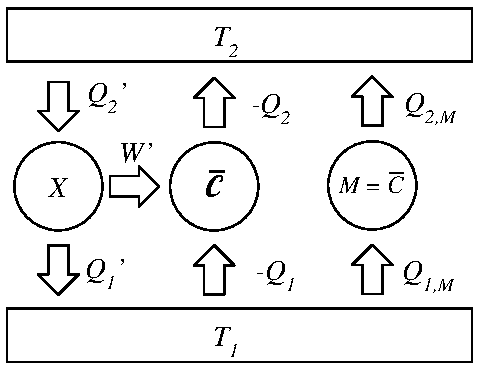
\includegraphics[width = \marginparwidth]{violare_carnot.pdf}
    \caption{Dimostrazione del primo enunciato del teorema di
    Carnot.}
    \label{teo_carnot}
\end{marginfigure}

La macchina di Carnot è per definizione reversibile. Esiste dunque
la sua versione frigorifera $\overline{\mathcal{C}}$ che opera al contrario.
$\overline{\mathcal{C}}$ avrà bisogno di lavoro esterno $-W$ per operare,
prelevando dalla sorgente fredda il calore $-Q_1$ e cedendo nel
complesso $-Q_2$ a quella calda. Immaginiamo che le due macchine
vengano ora accoppiate, in modo che $X$ alimenti $\overline{\mathcal{C}}$.
Ciò che ne deriva è una macchina $M$ che compie un certo lavoro
$W_M = W' - W$ e scambia certe quantità di energia con le sorgenti
tali che $Q_{1,M} = Q_1'-Q_1$ e $Q_{2,M} = Q_2' - Q_2$. $X$ è infine
progettata cosicché $W' = W$, cioè essa fornisce il lavoro di cui
$\overline{\mathcal{C}}$ ha bisogno. Ciò a cui vogliamo arrivare è
confrontare le efficienze a parità di lavoro prodotto.
Se allora si sostiene che $\eta_X > \eta_\mathcal{C}$ (attenzione che
ora torniamo a considerare $\mathcal{C}$! Possiamo farlo per supposizione
di reversibilità), ciò equivale
ad assumere che $W/Q_2' > W/Q_2$ da cui $Q_2 > Q_2'$. Come ci si
aspetterebbe, a parità di lavoro prodotto, $X$ consuma meno calore di
quello che invece utilizzerebbe $\mathcal{C}$.
Però in $M$ sta accadendo qualcosa che non dovrebbe: infatti
avremmo $Q_{2,M} < 0$, $W_M = 0$ e pertanto $Q_{1,M} > 0$. $M$ è proprio
una macchina che viola il secondo principio della
termodinamica secondo la formulazione di Clausius, perché non accade
altro che un trasferimento di calore dalla sorgente fredda a quella calda.
Purtroppo per chi ha puntato su $X$, si conclude che \[ \eta_X \leq \eta_\mathcal{C} \]

Se poi si assume che anche $X$ è reversibile, risulta che
$\eta_X \geq \eta_\mathcal{C}$ (basti ripercorrere la dimostrazione
sostituendo $X$ con $\mathcal{C}$), da cui si dimostra facilmente
che \[ \eta_X = \eta_\mathcal{C} \] Da questa conclusione, con
la quale termina la dimostrazione dell'intero teorema di Carnot,
si può osservare che la macchina di Carnot e tutte le macchine
reversibili che operano tra le stesse temperature sono equivalenti
in termini di efficienza; pertanto, la dimostrazione potrebbe essere
ripetuta anche senza limitarsi alla specifica macchina di Carnot,
eliminando, come proprio voleva Carnot, le particolari ``implementazioni''
che potrebbero rendere una macchina diversa dall'altra.

Nel caso $X$ non fosse reversibile, ciò significherebbe che
nessuna macchina reversibile può raggiungere, né tantomeno
superare, l'efficienza della corrispondente macchina di Carnot
che opera tra le medesime sorgenti. Non importa la macchina,
le sue prestazioni energetiche saranno sempre limitate superiormente
secondo l'espressione $1 - T_1/T_2$.

\subsection{Osservazioni di Carnot}
Da Carnot è possibile osservare che, se $Q_1 < 0$ è il calore ceduto
alla sorgente fredda e $Q_2 > 0$ quello assorbito dalla sorgente
calda, per le definizioni alternative di rendimento vale

\[ 1 + \frac{Q_1}{Q_2} \leq 1 - \frac{T_1}{T_2} \]

\noindent Che ci porta a concludere con la seguente:

\begin{align}
    \frac{Q_1}{T_1} + \frac{Q_2}{T_2} \leq 0
\end{align}

\noindent Ovviamente l'uguaglianza vale solo per macchine reversibili.
A prima vista, questa disuguaglianza potrebbe non comunicare
alcunché di straordinario. Nei prossimi paragrafi vedremo che
proprio da questa innocua relazione trarremo l'osservazione
forse più inquietante ma allo stesso tempo affascinante di
questo corso.

Un'altra osservazione: la seconda proposizione del teorema di Carnot
è molto importante, perché ci assicura, almeno sul piano teorico, che
le leggi della termodinamica valgono indipendentemente da come costruiamo
la nostra macchina, anche se questa non esiste ancora!

\section{Esperienza di Clausius; Entropia}
Un ulteriore personaggio degno del titolo di \textit{main character}
della termodinamica è il tedesco Rudolf Clausius, il quale estese
gli studi di Carnot. Di fatto, il teorema di Carnot non è sufficientemente
generale, è ancora distante dalla nostra realtà, perché nelle trasformazioni
Carnot impone la presenza di due sole sorgenti distinte. Illustriamo nel seguito
il teorema di Clausius, che apre la strada ad uno degli ultimi concetti di questi
appunti: l'entropia.

\subsection{Teorema di Clausius}
Abbiamo visto che una delle relazioni ottenute da Carnot è la
somma di rapporti $Q_1/T_1 + Q_2/T_2 \leq 0$. Ciò vale per tutte
le macchine, reversibili o meno, che operano tra due sorgenti 1
e 2 tali che $T_1 < T_2$. Avere però solamente due sorgenti è
alquanto limitante e irrealistico, perché nella realtà le macchine
operano su cicli ben più complessi, fluttuando tra svariati valori
di temperatura, come se operassero tra infinite sorgenti. Clausius
ebbe così la brillante idea di generalizzare le conclusioni di
Carnot per un ciclo termodinamico qualsiasi.

Si consideri il ciclo motore mostrato in figura. Esso attraversa
un infinità di temperature differenti. Immaginiamo di approssimare
la curva di questo ciclo mediante piccole trasformazioni adiabatiche
e isoterme. Se estendiamo queste piccole trasformazioni, otterremo
una griglia che suddivide l'area interna del nostro ciclo in tanti
piccoli cicli di Carnot. Per il ciclo $i$-esimo, vale allora
$Q_{1,i}/T_{1,i} + Q_{2,i}/T_{2,i} \leq 0$. Sommando i rapporti di
tutti i cicli otteniamo

\[ \sum_i \left(\frac{Q_{1,i}}{T_{1,i}} + \frac{Q_{2,i}}{T_{2,i}}\right) \leq 0 \]

\noindent Questa relazione non ci dice ancora molto di straordinario,
anche se possiamo notare due fatti: i tratti adiabatici non coinvolgono
scambi di calore per definizione e dunque possiamo ignorarli nel
nostro calcolo, perché il rapporto calore-temperatura è sempre nullo
durante questo tipo di trasformazione; esistono poi molti tratti
isotermi che vengono percorsi in versi opposti da cicli adiacenti.
Ciò accade nei tratti interni alla curva originale e non introducono
contributi calorici. Gli unici tratti di nostro interesse sono
quelli delle trasformazioni isoterme ai bordi del ciclo. Possiamo
allora riformulare la somma unendo solamente i rapporti di questi
tratti. Supponendo che il tratto $j$-esimo sia una isoterma che
costituisce parte del bordo della curva originale, vale
$\sum_j Q_j/T_j \leq 0$. Più elegantemente, passando all'infinitesimo
si ottiene la seguente disuguaglianza

\begin{align}
    \oint \frac{dQ}{T} \leq 0
\end{align}

\noindent che è proprio la tesi del teorema di Clausius. L'integrale
prende il nome di \textit{integrale di Clausius}. Il caso particolare
dell'uguaglianza vale solamente per trasformazioni reversibili.

\subsection{Variazione di entropia}
Si consideri una trasformazione termodinamica \textit{reversibile} qualsiasi.
Per ipotesi di reversibilità, l'integrale di Clausius calcolato sulla curva $\tau$
di tale trasformazione nel piano pressione-volume è nullo.

\[ \oint_\tau \frac{dQ}{T} = 0 \]

\noindent Selezioniamo due punti, $A$ e $B$, distinti su questo ciclo. Scomponiamo
dunque l'integrale nei due percorsi, sempre reversibili, $\alpha$ e $\beta$.

\[ \int_{A,\alpha}^{B} \frac{dQ}{T} + \int_{B,\beta}^{A} \frac{dQ}{T} = 0 \]

\noindent Trattandosi di un ciclo reversibile, vale la proprietà antisimmetrica
dell'integrale. Giungiamo dunque alla seguente conclusione:

\[ \int_{A,\alpha}^{B} \frac{dQ}{T} = \int_{A,\beta}^{B} \frac{dQ}{T} \]

\noindent Dunque, qualsiasi sia il percorso tra $A$ e $B$, l'uguaglianza
precedente vale sempre per percorsi reversibili. Vi è dunque una dipendenza
di una certa quantità dai soli stati iniziale e finale della trasformazione.
Definiamo, in modo simile all'energia potenziale studiata in meccanica,
la differenza di entropia tra due stati termodinamici.

\begin{align}
    \Delta S_{AB} \stackrel{\text{def}}{=} \int_{A,\text{rev}}^{B} \frac{dQ}{T}\label{variaz_entropia}
\end{align}

\noindent Definiremo solamente la differenza, non l'entropia in sé.
Sappiamo però che l'entropia è una funzione di stato, come abbiamo
potuto vedere poco prima. Da un punto di vista dimensionale, l'entropia
è un semplice rapporto tra energia e temperatura, una sorta di
indice della quantità di calore scambiato ad una data temperatura.
Durante gli scambi energetici, però, spesso la temperatura dei corpi
coinvolti cambia. Possiamo approssimare questi fenomeni immaginando
infinitesimi quanità di calore che vengono scambiate di volta in volta
a temperature diverse:

\begin{align}
    dS \eqdef \left[\frac{dQ}{T}\right]_\text{reversibile}\label{entropia_infinitesima}
\end{align}

\subsubsection*{Cos'è l'entropia?}
Facciamo presente che in questo corso definiamo solamente la variazione
di entropia, non l'entropia assoluta di un sistema, un po' come si fa
con l'energia potenziale. Però, rispetto a quest'ultima, l'entropia
può essere definita (si vedano gli approfondimenti per brevi accenni,
in particolare la definizione \ref{entropia_meccanica_statistica}) ma
per i nostri scopi non è molto utile.


\subsubsection*{Variazione di entropia in trasformazioni fondamentali}
Possiamo aggiungere la variazione di entropia a tutte quelle equazioni viste nelle
trasformazioni termodinamiche fondamentali. Supponiamo come sempre
che tali trasformazioni siano quasistatiche reversibili. Applichiamo
le definizioni \ref{variaz_entropia} e \ref{entropia_infinitesima},
quindi per ogni trasformazione cerchiamo il calore $dQ$ e
la temperatura alla quale esso viene scambiato, riconducendoci
in alcuni casi a relazioni che legano il calore con la temperatura
stessa per ottenere funzioni da integrare, passando da $dS$ a $\Delta S$.

\begin{itemize}
    \item \textbf{Isoterma:} nelle isoterme abbiamo scoperto che
    $dQ = nRTdV/V$. Ci basta dividere questo calore per la temperatura
    alla quale sta avvenendo la trasformazione, ottenendo dunque
    
    \begin{align}
        dS_\text{isoterma} = nR\frac{dV}{V}
    \end{align}

    \noindent Integrando, otteniamo

    \begin{align}
        \Delta S_{AB} = nR\ln\left(\frac{V_B}{V_A}\right)
    \end{align}

    \noindent Possiamo notare che, in una isoterma, $\Delta S_{AB} > 0 \Leftrightarrow V_B > V_A$.
    Ciò è compatibile con l'intuizione dell'idea di entropia: se il gas
    si ``sparge'' in un volume maggiore, il suo disordine è maggiore e
    dunque aumenta la sua entropia.

    \item \textbf{Isocora:} dalla nostra tabellazza sappiamo che $dQ = nc_VdT$,
    quindi

    \begin{align}
        dS_\text{isocora} = nc_V\frac{dT}{T}
    \end{align}

    \noindent da cui

    \begin{align}
        \Delta S_{AB} = nc_V\ln\left(\frac{T_B}{T_A}\right)
    \end{align}

    \noindent In questo caso, $\Delta S_{AB} > 0 \Longleftrightarrow T_B > T_A$.
    Intuitivamente, il disordine del sistema aumenta per via dell'incremento
    di temperatura. Immaginando un gas ideale (ma anche un cubetto di ghiaccio
    in una tazza di té, the, htegh, o come si scrive), di fatto le particelle
    si agitano di più e il sistema diventa più caotico.

    \item \textbf{Isobara:} vale $dQ = nc_pdT$ e allora
    
    \begin{align}
        dS_\text{isobara} = nc_p\frac{dT}{T}
    \end{align}

    \noindent e allora

    \begin{align}
        \Delta S_{AB} = nc_p\ln\left(\frac{T_B}{T_A}\right)
    \end{align}

    \noindent La spiegazione intuitiva è pressoché la stessa di
    quelle precedenti. Anzi, da un certo punto di vista si tratta
    proprio di una combinazione delle prime due.

    \item \textbf{Adiabatica:} abbiamo $dQ = 0$.
    
    \begin{align}
        dS_\text{adiabatica} = 0
    \end{align}

    \noindent da cui ovviamente segue che $\Delta S_{AB} = 0$.
    In questa trasformazione la spiegazione intuitiva del
    binomio entropia-disordine è più complessa. Per andare al punto,
    immaginiamo una compressione adiabatica di un gas: il suo
    volume diminuisce, quindi saremmo tentati di concludere che
    l'entropia del sistema diminuisce, ma in realtà in una adiabatica
    deve aumentare anche lìenergia interna del gas, quindi anche la
    sua temperatura. Precedentemente abbiamo associato l'aumento di
    temperatura all'aumento di entropia. Perciò il disordine dovuto
    alla temperatura che si innalza compensa l'ordine che si introduce
    col volume. Il ragionamento è analogo per una decompressione
    adiabatica.
\end{itemize}

\noindent Aggiungiamo una formula bonus, la \textbf{variazione di
entropia in transizioni di fase}. Ricordiamo che, in un cambiamento
di fase (immaginiamo il ghiaccio che si scioglie, da solido a liquido),
bisogna fornire al sistema una certa quantità di calore proporzionale
alla massa che si intende trasformare. Questo è il calore latente,
che dipende da una costante $\lambda$. Allora possiamo scrivere
$dQ = \lambda dm$, ovvero una piccolissima quanità di calore che
permette ad una piccolissima quantità di massa di trasformarsi.
Concludiamo che

\begin{align}
    dS_\text{tfase} = \frac{\lambda dm}{T}
\end{align}

\noindent Ricordiamo anche che le transizioni di fase avvengono
(idealmente) a temperature costanti. Allora

\begin{align}
    \Delta S_{AB} = \frac{\lambda m}{T}
\end{align}


\subsubsection*{Diagramma temperatura-entropia}







\subsection{Il teorema dell'entropia}



\subsubsection{Che dire dei frigoriferi?}






\section{Approfondimenti}
Questo pacco di termodinamica si conclude, ma essendo grande
merita molti approfondimenti.

\subsection{La questione del calorico}
La fisica poggia su un substrato filosofico molto sofisticato e
sviluppato, dal quale hanno origine, per esempio, molte interpretazioni
della realtà che viene studiata. Una questione che segnò le ricerche
nel campo della termodinamica fu quella di definire e chiarire le
ragioni d'essere del \textit{calore}, ovviamente avanzando ipotesi
secondo il metodo scientifico.

Prima di Joule, si parlava in letteratura di \textit{calorico},
qualcosa che veniva interpretato come un fluido vero e proprio,
dotato di esistenza propria e in grado di muoversi da corpo a
corpo, da sorgenti più calde a quelle più fredde. La temperatura
veniva poi definita sulla base della concentrazione di calorico
in un certo corpo, anche se calore e temperatura rimanevano in
molti casi concetti confusi, come a volte capita anche nell'esperienza.

Grazie agli esperimenti di Joule, la fisica comprese che il calore
rappresenta in realtà una forma di energia, qualcosa che
non esiste in natura, ma che la descrive. Nell'esperimento del
mulinello, l'innalzamento di temperatura dell'acqua è dovuto al
lavoro compiuto da una massa in caduta. Secondo l'interpretazione
precedente, del calorico sarebbe comparso dal nulla, quando invece
viene semplicemente osservata una trasformazione di lavoro in calore,
in accordo con i principi di conservazione già sviluppati in meccanica.


\subsection{Espansione libera dei gas}



\subsection{Micro- e macro-stato}
Con i nostri strumenti non siamo in grado di definire l'entropia in
senso assoluto, ma solo la sua variazione. Studi più avanzati,
collegati alla cosiddetta \textit{meccanica statistica}, consentono
invece di esprimere in forma chiusa l'entropia di un sistema.

\begin{align}
    S \eqdef k_B \ln [N]\label{entropia_meccanica_statistica}
\end{align}

\noindent dove $k_B$ è la costante di Boltzmann, mentre $N$
corrisponde al \textit{numero di microstati compatibili con il
macrostato}. Vediamo cosa si intende con questa definizione,
mostrando un esempio molto celebre: supponiamo di avere due
scatole, $A$ e $B$, suddivise ciascuna in 6 scompartimenti
identici. In ogni scompartimento, o slot, può essere collocata
una sola pallina tra un mucchio di altre, identiche e indistinguibili
tra loro. La particolarità
di queste palline è la loro insolita abitudine di rimbalzare
da uno slot all'altro in maniera del tutto casuale ed imprevedibile.
Immaginiamo che la scatola $A$ contenga
un totale di 4 palline, mentre $B$ due. Se avviciniamo $A$ e
$B$, le palline cominceranno a saltare non solo negli slot
della stessa scatola ma anche in quelli dell'altra. La situazione è
mostrata in figura \ref{micromacro}. Il macrostato del sistema
costituito dalle due scatole $A$ e $B$ e dalle loro palline,
in totale 6, è descrivibile dalla proprietà \textit{numero di palline nella scatola $X$},
dove $X = A, B$. Per macroscopico intendiamo
il fatto di non essere per nulla interessati di dove si trovano
le palline in ciascuna scatola, ma solamente di conoscere il
loro numero totale, in $A$ o in $B$. Il microstato, invece,
è rappresentato dalla configurazione delle palline negli slot.

\begin{marginfigure}
    \centering
    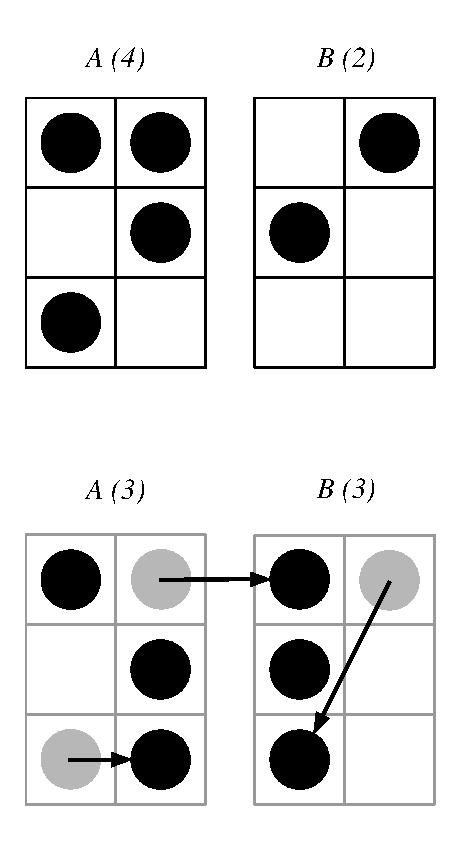
\includegraphics[width = \marginparwidth]{micro_macro_stati.pdf}
    \caption{Rappresentazione dei microstati dell sistema di scatole
    $A$-$B$. In alto viene mostrata la situazione iniziale, in cui
    un particolare microstato determina il macrostato \textit{4 palline
    in $A$ e 2 in $B$}. In basso, il sistema passa ad un nuovo microstato.
    Notare che le palline possono muoversi anche tra le scatole; infatti,
    il macrostato diventa \textit{3 palline in $A$ e 3 in $B$}.}
    \label{micromacro}
\end{marginfigure}

Poniamoci ora la domanda: quanti microstati sono compatibili
col macrostato \textit{4 palline in $A$, 2 in $B$}? Per rispondere,
ci basta applicare un pizzico di combinatoria\footnote{Ricorriamo
al metodo del coefficiente binomiale. Per ciascuna scatola, possiamo immaginare
di assegnare gli $n = 6$ slot alle $k$ palline del macrostato. Però, dal
momento che le palline sono tra loro indistinguibili, non dobbiamo incappare
nell'errore di contare configurazioni per le quali, scambiando due qualsiasi
palline, gli slot occupati sono sempre gli stessi. Il coefficiente binomiale
tiene conto di questo fatto senza contare eventuali configurazioni uguali,
ed è definito come $\binom{n}{k} = \frac{n!}{k!(n - k)!}$. Per finire, dato
che ci interessa conoscere le configurazioni totali del sistema scatola-$A$-scatola-$B$,
dobbiamo applicare il principio del calcolo combinatorio e moltiplicare tra
loro i coefficienti binomiali.},
determinando quante sono le configurazioni di 4 palline in 6 slot di $A$
e 2 in 6 slot di $B$. I microstati sono in tutto

\[ N_{4,2} = \binom{6}{4} \cdot \binom{6}{2} = 225 \]

Ora, poniamo vicine tra loro $A$ e $B$ e lasciamo che le palline
saltino tra l'una e l'altra scatola. Quante possibilità esistono
per cui vale il macrostato \textit{1 pallina in $A$, 5 in $B$}?
Ancora, la combinatoria ci fornisce il risultato

\[ N_{1,5} = \binom{6}{1} \cdot \binom{6}{5} = 36 \]

\noindent Notiamo immediatamente una cosa: il numero di microstati
compatibili è decisamente più piccolo. Proviamo a fare un ultimo
calcolo, contando invece i microstati per cui sono presenti
\textit{3 palline in $A$ e 3 in $B$}, ovvero le palline sono
equamente distribuite tra le due scatole:

\[ N_{3,3} =\binom{6}{3}^2 = 400 \]

In virtù della definizione \ref{entropia_meccanica_statistica}, possiamo concludere che
l'entropia del sistema con la configurazione 4-2, quella iniziale,
è minore di quella 3-3.
Dal momento che le palline si muovono tra gli slot in maniera
casuale, possiamo supporre che tutte le configurazioni possibili
siano equiprobabili, ma molte di esse, che sono singoli microstati,
corrispondono agli stessi macrostati. È dunque più probabile che
le palline si dispongano per lo più equamente tra $A$ e $B$
anziché disporsi tutte in una sola delle due, come i calcoli
rivelano. Se aumentiamo
le palline e gli slot, tra l'altro, il numero di microstati
vicini a quello in cui le palline sono esattamente divise
cresce esponenzialmente. Per la meccanica statistica, questo
è il motivo per cui i sistemi termodinamici tendono a massimizzare
la propria entropia. Ma questo non è dovuto al fatto che essi
``vogliono'' farlo, bensì perché è il destino più probabile.

Non abbiamo scelto l'analogia delle palline e delle scatole a caso.
Possiamo immaginare le palline come particelle di gas e le scatole
come contenitori dotati di volume, occupabile dalle particelle stesse
in svariate configurazioni. Oppure, le scatole possono essere
due barre di metallo, una calda e una fredda, e le palline
rappresentano i ``pacchetti'' di energia con i quali si può
quantificare il calore scambiato, oltre la temperatura delle barre durante
gli stati di equilibrio. Come già concluse Boltzmann, non è
del tutto vero che è impossibile che il gas si accatasti
tutto in un solo contenitore, oppure che il calore fluisca
dal corpo freddo a quello caldo. Nulla vieta il verificarsi di
certi fenomeni. Semplicemente, è estremamente
improbabile che ciò accada e questo vale ancor di più per sistemi
sempre più grandi e complessi, proprio quelli in cui viviamo noi.
Ricordate la famosa, apparentemente innocua osservazione scritta
all'inizio della sezione sul secondo principio? Ora dovrebbe essere
evidente l'importanza di quel \emph{mai spontaneamente}.

\subsubsection*{Entropia, disordine, informazione, tempo}
L'entropia non è propriamente qualcosa che esiste fisicamente,
ma è solo uno stratagemma matematico per mettere in luce una
certa regolarità del mondo.
Ma per noi umani, cos'è allora l'entropia? Alla luce di questa breve introduzione
alla meccanica statistica, non si tratta altro che una descrizione
del grado di disordine di un sistema: più i costituenti di un
sistema sono sparsi, disordinati, più l'entropia aumenta. Questo
è il motivo per cui il concetto di entropia trova svariati campi
d'applicazione al di fuori della fisica, tra le quali anche
l'informatica. Uno spunto interessante che ha permesso l'entropia
di avere successo in altre branche del sapere è il seguente: un
sistema disordinato richiede maggior informazione per essere
descritto rispetto ad uno ordinato, per via dei diversi gradi
di complessità che si possono presentare, come abbiamo visto
nell'esempio delle palline.

Come già emerge dal teorema dell'entropia, esiste una quantità
che varia in maniera differente a seconda del verso con cui il
tempo scorre. La nostra percezione del tempo è abituata a vedere
il succedersi degli eventi nella sequenza più naturale e spontanea
che esiste in natura, ovvero quella per cui i sistemi fisici tendono
a gradi di disordine sempre maggiori.

\subsection{Il terzo principio}
Ebbene sì: esiste un terzo principio della termodinamica che è stato
ignorato in queste lezioni. Esso introduce concetti già avanzati, ma,
in alcune delle sue formulazioni equivalenti, rimane comunque estremamente
affascinante. In breve, questo principio afferma che non esiste
temperatura più bassa dello zero assoluto e che quest'ultimo non è
neppur raggiungibile. Ecco una delle formulazioni:

\begin{center}
    \textit{Non esiste processo in grado portare la temperatura di un corpo\\allo
    zero assoluto tramite un numero finito di passi.}
\end{center}

\noindent Analogamente alle dimostrazioni viste per l'equivalenza
degli enunciati del secondo principio, anche il terzo può essere
dimostrato con un esperimento mentale che si basa sullo stesso principio
di funzionamento del frigorifero:

Supponiamo di avere un insieme di oggetti a 0 K e un oggetto $X$ da
raffreddare e a temperatura superiore. Mettiamo $X$ in
contatto termico con uno degli oggetti a 0 K. Sappiamo dalla calorimetria
che i due corpi raggiungeranno l'equilibrio termico e avranno una
temperatura uguale intermedia alle loro iniziali. Possiamo allora
ripetere il raffreddamento con $X$ e un altro oggetto a 0 K, ma
non raggiungeremo mai lo zero assoluto con un numero finito di
contatti, perché l'equilibrio termico viene raggiunto ad una temperatura
che è sempre compresa tra 0 K (escluso) e quella di $X$ raffreddato, che
è maggiore di 0 K.

Purtroppo per noi, non è ancora stato trovato un oggetto a 0 K\footnote{Sono
molti gli oggetti leggendari come questo in fisica: la massa infinita, il
corpo nero, il piano privo di attrito...}, né tantomeno sono state
trovate tecniche di raffreddamento in grado di raggiungere lo zero
assoluto, anche se siamo stati in grado di avvicinarci ad esso
nell'ordine di una frazione di Kelvin.


\subsection{Macchine e moto perpetuo}
Parlando di principio secondo, abbiamo ipotizzato l'esistenza di macchine
in grado di convertire l'energia fornita (il calore) in lavoro senza alcuna
dissipazione o perdita. Per via del secondo principio questo non è possibile
e ci siamo rassegnati presto ad esso. Ora che però siamo nella sezione approfondimenti,
possiamo fantasticare quanto ci pare: e se non valesse il secondo principio
della termodinamica? Per il primo principio, sarebbero ammesse le leggendarie
macchine super efficienti, che una volta azionate entrerebbero in un regime
di funzionamento conosciuto come moto perpetuo.

Una macchina capace di moto
perpetuo è in grado di produrre lavoro senza alcun apporto di energia esterno,
eccetto quello necessario ad azionarla. Ricordando sempre il caro, vecchio primo
principio, $\Delta U = Q - W$, sappiamo che $\Delta U = 0$ per via del
funzionamento ciclico delle macchine, da cui $W = Q$. $Q$ rappresenta l'energia
iniziale che innesca il moto, mentre $W$ è il lavoro prodotto. Attenzione però,
perché anche il primo principio pone un limite a queste macchine.
Dal momento che calore e lavoro si equivalgono, il moto perpetuo dovrebbe
convertire queste due forme di energia in continuazione. In altre parole,
la macchina può solo autoalimentarsi e non potremo mai sfruttarla per generare
energia infinita, pena lo spegnimento della macchina stessa.

Nella storia (anche in tempi recenti) sono state numerose le proposte
di macchine del genere, ma ovviamente nessuna di esse funziona.
Sottolineamo che il fantomatico moto perpetuo, \emph{prima o poi}, è
destinato a fermarsi. Non viene specificato dopo quanto tempo, che tuttavia
è sicuramente finito: una frazione infinitesima di secondo, un minuto,
un'ora, un anno, una decina di miliardi di anni.
Ecco alcuni esempi fantasiosi di moto perpetuo:

\begin{itemize}
    \item Il mulino: un mulino ad acqua aziona una pompa idraulica,
    che riporta il liquido in cima alla ruota, che quindi gira e
    produce lavoro per mantenere l'acqua in circolo e far ruotare
    sé stessa indefinitamente.

    \item La lampadina: una lampadina emette la stessa luce necessaria
    ad attivare dei pannelli fotovoltaici che la alimentano.

    \item Contenitore di Boyle: un vaso riempito di acqua possiede
    un tubo che dal fondo convoglia l'acqua in cima al contenitore.
    Il tubo è estremamente stretto e allungato mano a mano che si
    raggiunge l'estremità. Questa macchina idraulica dovrebbe permettere
    all'acqua di scorrere all'infinito nel tubo, ritornando nel
    vaso come una fontanella, perché per capillarità (per questo il tubo deve esssere molto
    stretto) il liquido dovrebbe essere risucchiato. Per svariate
    qestioni di pressione e fluidodinamica, la fontanella non
    riuscirà mai a scorrere.
\end{itemize}

Questi esempi mostrano che i principi della termodinamica non
sono validi solamente in quei sistemi in cui si trattano caldo,
freddo e così via. Come Carnot previde, le leggi reggono anche
per macchine costruite nelle maniere più bizzarre.